%%%%%%%%%%%%%%%%%%%%%%%%%%%%%%%%%%%%%%%%%
% Sleek, Extensible Journal Article
% LaTeX Template
% Version 0.1
% Date 01/05/2014
%
% Original author:
% Calem Bendell
%
% License:
% CC BY-NC-SA 3.0 (http://creativecommons.org/licenses/by-nc-sa/3.0/)
%
%%%%%%%%%%%%%%%%%%%%%%%%%%%%%%%%%%%%%%%%%

\documentclass[10pt, twocolumn]{scrartcl}
\usepackage[T1]{fontenc}

\usepackage{lipsum}

\usepackage{kpfonts}
\usepackage{helvet}
\linespread{1.05}
\usepackage{microtype}

\usepackage[top=5em, left=5em, right=5em, bottom=7em, columnsep=2em]{geometry}
\usepackage[hang, small,labelfont=bf,up,textfont=it,up]{caption}
\usepackage[hidelinks, colorlinks=true]{hyperref}
\usepackage{booktabs, float, paralist, titlesec, abstract, titling, enumitem, graphicx}
\usepackage[usenames,dvipsnames,svgnames,table]{xcolor}
\usepackage[flushmargin,hang,multiple]{footmisc}
\interfootnotelinepenalty=10000

\renewcommand{\abstractnamefont}{\normalfont\large\sffamily}
\renewcommand{\abstracttextfont}{\normalfont\itshape}

\titleformat*{\section}{\Large\sffamily}
\titleformat*{\subsection}{\large\sffamily}
\titleformat*{\subsubsection}{\itshape\sffamily}
\titleformat*{\paragraph}{\large\bfseries\sffamily}
\titleformat*{\subparagraph}{\large\bfseries\sffamily}

\setlist[description]{format=\normalfont\itshape}

\renewcommand{\maketitle}{\noindent\rule{\linewidth}{1pt}\LARGE \vspace{1em} \newline
\sffamily \scshape \thetitle \\
\normalfont \sffamily  \theauthor \\
\thedate
\newline\noindent\rule{\linewidth}{1pt}
\normalfont
\normalsize}


\title{Automation Team Research Review}
\author{
\normalsize
{ Calem Bendell, Shalon Liu, Han Yang Zhao} \\
Hyvedev, McGill University \\
\href{mailto:calem.bendell@mail.mcgill.ca}{calem.bendell@mail.mcgill.ca}
}
\date{}

\begin{document}
\maketitle

\begin{abstract}
The automation team has already made the majority of the decisions it needs to make through research and some experimentation.
This is a summary of progress, research, and decisions made...
annnd.. i'll fill this in as i get to it.
\end{abstract}

\begin{center}
	
\includegraphics[width=.3\textwidth]{gfx/hyvedev-logo.pdf}
\end{center}

\begin{multicols}{2}

\section{Introduction}

	Sustainability comes in many forms, some easier than others.
	In most instances, people want to be sustainable, they just also don't want to be inconvenienced.
	It is the automation team's goal to provide sustainability in a feasible fashion by providing it "cloaked" in convenience through HyveOS.
	
	HyveOS is a software that implements a platform to receive and send data from a house. 
	Data is collected by cameras and microphones placed in public rooms, to which the occupants can issue commands, and received through already owned phones or speakers in the house.
	
	The primary goals for HyveOS are:
	\begin{description}
		\item[Safety] making houses capable of detecting dangers such as a burglary or an occupant falling down and not getting back up
		\item[Cooperativity] allowing houses to balance each other's energy loads and resources
		\item[Sustainability] letting neighbours to connect with each other and share their own resources, such as tools and food, more easily (and with encouragement from their houses)
		\item[Hands-Free Operation] enabling people to connect fluidly to the world of data around them through motion tracking systems more accurate than Microsoft's Kinect
		\item[Community] gently encouraging neighbours to make connections and share with each other
	\end{description}

	\subsection{Decisions Made}
	
		The decisions described in Table \ref{decision-matrix} have already been made to differing degrees of certainty.
		
	\subsection{Requested Feedback}
	
		In our case most of the technological decisions have been fairly firmly made.
		We were able to do this through extensive research and with the knowledge that what we do can be done fairly independently of the other Solar Decathlon teams.
		
		What feedback we do request is where you see automation fitting in with your part of the house.
		Also I would like to know whether or not you think HyveOS should increase or decrease the scope of its goals or if you think our goals are misguided.


\end{multicols}
		\begin{table}[h]
			\centering
			\begin{tabular}{c|r|r}
				\toprule
					Aspect & Decision & Firmness (0-5) \\
				\midrule
					Satellites Hardware & Raspberry Pi & 5 \\
					Server Hardware & Custom PC Rig & 4 \\
					Automation Satellites & Arduino & 2 \\
					Satellite Operating System & Ubuntu Server & 4 \\
					Satellite Peripherals & Audio, Visual & 2 \\
					Primary Interface & Website (with mobile) & 4 \\
					Primary Language & NodeJS & 4 \\
					Analytical Language & Python & 4 \\
					\bottomrule
			\end{tabular}
			\label{decision-matrix}
			\caption{A tabular description of some of the decisions already made.}
		\end{table}
\begin{multicols}{2}		

\section{Background}

	\subsection{Servers and Satellites}
	
	\subsection{The Internet of Things}
	
	\subsection{The DIY Hardware Movements}

\section{Research}

	\subsection{Hardware}
	
		Most of hardware concern comes down to Arduino vs Raspberry Pi vs TI Launchpad vs Beaglebone, some of which are depicted in Figure \ref{fig:pi-arduino-beaglebone}. 
		For now, TI Launchpad and Beaglebone will be discounted, though the TI Launchpad is perhaps interesting in that it has the backing of a very large company and is desperate to gain market share.
		
		This distinction is more made at what Hyvdev aims to do.
		The following quote from James Bruce clarifies the intended purposes of each of these machines.
		
		\begin{quote}
			The Arduino runs the Arduino firmware, a basic bit of core software which allows it to communicate with a computer over USB and gives access to all the features. You generally wouldn't replace this firmware, but it is possible. Once your application has been loaded, you can just plug it in anywhere and it'll start working immediately, you don't need to reboot, plug in a keyboard, or choose an application to run. It does the one job it's been programmed to do, and it does it immediately.
			
			The Raspberry Pi on the other is a complete, functional, mini-computer. It requires an operating system - the first thing you need to choose that will dramatically affect your experience - and has all the bits and pieces you might expect a full computer to have (just in a smaller scale). Storage is provided from a micro-SD card, while built-in Ethernet allows for networking (you can get networking on Arduino too, but it requires an add-on "shield").
		\end{quote}
		
		If the Arduino is chosen, then the team chooses its focus is more on typical home automation, such as controlling windows and doors and doing basic home monitoring; alternatively, the Raspberry Pi signifies a much more involved automation process.
		
		The Raspberry Pi was chosen to empower the team to provide a full automation experience, attempting to make the "smart home."
		As it turns out, a few other groups are also attempting to make the smart home, Nest not the least of them.
		It is thus our job to also distinguish ourselves from these competitors.
		
		But really, why choose?
		We can use both, using the Arduino (or TI Launchpad) to control much of the typical home automation and the Raspberry Pi for controlling satellites.
	
	\subsubsection{Raspberry Pi}
	
	\subsubsection{Arduino}
	
		The Arduino is a single-board microcontroller that is generally described as perfect for electronics projects. 
		The board has exposed I/O pins for use by other circuits or sensors.
		A simple example of input and output control that the Arduino can do is translating input from a sensor, such as key presses, to outputs, such as a musical note as long as the keyboard and speakers are attached.
		Arduino can be programmed from a regular computer, connected via a USB port, which acts also a power source.
		
		Some of the main advantages of using Arduino is both its hardware and software are open source and the Arduino software runs on Windows, Mac and Linux, so it can be programmed from almost any operating system.
		The Arduino community is actively developing and adding to the programming libraries. 	
		It is generally considered most suitable for rapid prototyping in research applications, not for industrial scale usage \footnote{On a slightly subjective note, while some seem to thin the Arduino inappropriate for industrial use, it is not because the Arduino is incapable in any way.  This is because the Arduino lacks some certifications and does not have an industry certified training program for its use, so one cannot find engineers "qualified" to use an Arduino.  Basically, there is no company supporting it from behind supporting the ecosystem of closed systems where everyone gets a piece of the pie, and because managers and human resources are frequently cowards who would prefer their company passes on blame whenever possible to other companies for hardware failures.  The "Programmable logic controller" has this market largely under wrap, with a few other big companies dominating the field.  It's a wasteful, cowardly, ridiculous situation, but it is what people will do to successfully dilute blame.  For a company to use the Arduino, they would have to accept full responsibility for any hardware issues and would also take it upon themselves to ensure they can find engineers who know how to work with the platform, a list that is apparently too frightening for large companies to bother with so they instead endure the steep costs of deeply entrenched solutions. \\ \emph{Calem}}.
		
		The simpler programming environment of Arduino can be seen both as an advantage and disadvantage.  
		It is a lower barrier of entry for non-electrical engineers to program but it does this by adding one layer of abstraction on top of C, which means you don't have control over every bit and byte of the less abstracted controllers.
		It is also impossible to fully customize the board as it doesn't not allow one to hand-solder components (which at this level, we shouldn't even be considering)
		Using the Arduino language decreases the portability of the code (not the hardware), so you'd be stuck with Arduino hardware.
		
		Overall, the Arduino board is very flexible with low barrier of entry for those just getting in to hardware hacking and lots of examples online.  Though it'd be good to keep in mind that Arduinos are good for small projects and prototyping (i.e. trying things out and experimenting).  As the teams advances and becoming more familiar with microcontrollers and requiring specialized function, the Arduino may not be suitable.
		
	\subsection{Load Balancing}
	
	\subsubsection{Specification}
		
		HyveOS will control and monitor the house's power usage using custom "appliance boxes." Appliance boxes will have appliances plug into them and will themselves plug into outlets. Each box will output a signal representing how much power the device is drawing, and would take as input a binary signal telling the box to allow the device to draw power (1) or to kill power to the device (0). If the appliances as a whole are drawing more power than the house is allowed (e.g. device A draws 100 Watts, device B draws 100 Watts, but the house can only use 150 Watts for whatever reason), the controller will kill some of the devices and only reactivate them when the total usage drops below a certain threshold. The "boxes" in practice might be built into our house's outlets.
		
	\subsubsection{Implementation}
	
		The house's main controllers (Raspberry Pis) will need to run threads that can manage the signals to and from the appliance boxes. The signals themselves will need either a wired or wireless communication channel. A wired channel will need wiring to connect to the main controllers' general-purpose I/O (GPIO) pins and possibly circuitry for signal refreshing and electromagnetic shielding. A wireless channel will require wireless transceivers for each appliance box. For ease of prototyping, we will use the Spark Core to receive controller input and transmit power usage output wirelessly, and we will use an open-source relay shield for the Spark Core to switch the appliance's "hot" wire (the wire which carries AC power supply voltage) from ground (if the device ought not draw power) or the box's hot wire.
		
	
\end{multicols}
\begin{figure}[H]
	\centering
	\caption{An Arduino, Raspberry Pi, and Beaglebone from left to right, demonstrating their relative size.  Their absolute size should be inferred by the size of their ports.}
	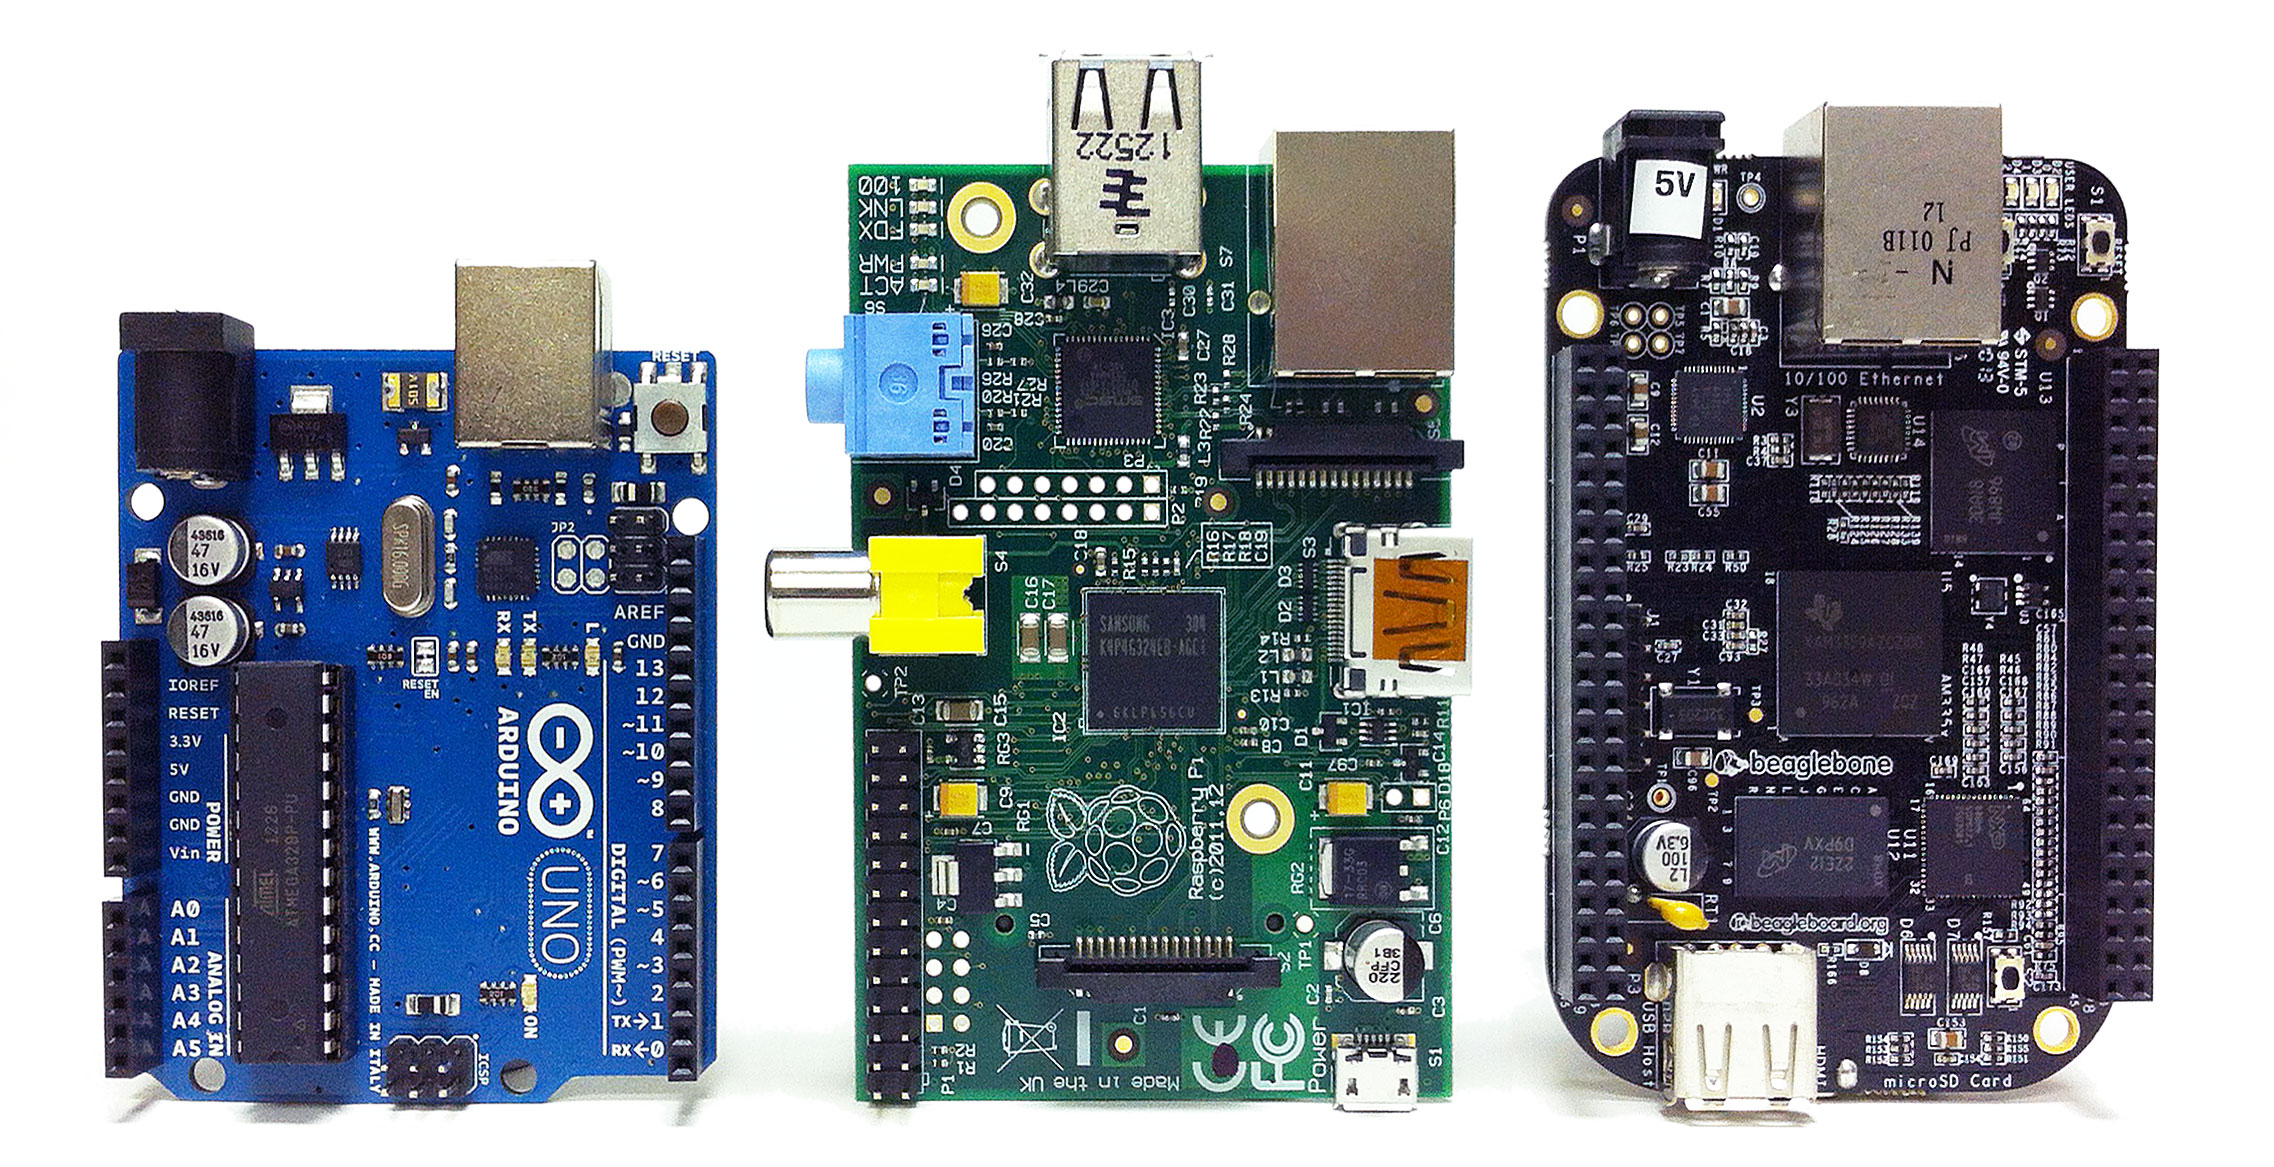
\includegraphics[width=.9\textwidth]{gfx/pi-arduino-beaglebone.jpg}
	\label{fig:pi-arduino-beaglebone}
\end{figure}
\begin{multicols}{2}
	
	\subsection{Software}
	
		It is in the software that Hyve is distinguishable.
		First, let's look at the competitors.
		\begin{description}
			\item[Nest] is a home automation company that designs and manufactures sensor-driven, Wi-Fi-enabled, self-learning, programmable thermostats and smoke detectors.
			\item[Insteon] is a home automation networking technology that enables light switches, lights, thermostats, motion sensors, and other devices to interoperate through power lines, radio frequency (RF) communications, or both.
			\item[Pointgrab] aims to control all household appliances with natural guestures.  Pretty damn cool, but not exactly competing with us yet.
			\item[Revolv] \$299 device that connects existing smart devices, unifying them to make a full smart home.
		\end{description}
		
		Nest gets a lot of hype, but is underwhelming from a home automation perspective.
		It is likely that they will make an aggressive shift into home automation since their purchase by Google.
		
		There are some other competitors, but most follow this tune.
		It is thus not difficult to see where Hyve can differ.
		
		These other approaches are largely cautious, timid, and realistic.
		Hyve is a student group, part of the Solar Decathlon competition.
		We do not need to be realistic at first.
		We do not need to be cautious.
		Fortunately, it is the sign of many great adventures (and successful companies) to not be overly concerned about what is considered normal today and instead be prepared for what is normal in the future.
		
		This brings us to Hyve's primary endeavour, which is behaviour modification and true integration of technology and home life, but this topic is saved for the conclusion.
		
	\subsection{Available Software}
	
		This is the most important section of the paper!
		Here is what's already out there.
		More importantly, this is what is available to use.
		
		\subsubsection{WiTrack: Through-wall 3D Tracking Using Body Radio Reflections}
		
			A technology from CSAIL at MIT.
			
			\begin{quote}
				WiTrack is a device that tracks the 3D motion of a user from the radio signals reflected off her body. It works even if the person is occluded from the WiTrack device or in a different room. WiTrack does not require the user to carry any wireless device, yet its accuracy exceeds current RF localization systems, which require the user to hold a transceiver. It transmits wireless signals whose power is 100 times smaller than Wi-Fi and 1000 times smaller than cellphone transmissions.
				
				WiTrack localizes the center of a human body to within 10 to 13 cm in the x and y dimensions (about the size of an adult hand), and 21 cm in the z dimension. It also provides coarse tracking of body parts, identifying the direction of a pointing hand with a median of 11.2 degrees. It can also detect falls with 96.9\% accuracy. WiTrack can be incorporated into consumer electronics and has a wide set of applications.
			\end{quote}
			
			The paper for the technology is available \href{http://witrack.csail.mit.edu/witrack-paper.pdf}{here}.
			
		\subsubsection{Wit Speech}
			
			Wit speech is one of several online APIs for voice recognition.
			It's a very attractive package, though perhaps not as good as Nuance's offerings yet.
			In any case, they provide an excellent description of their service:
			
			\begin{quote}
				Wit.AI enables developers to add a natural language interface to their app or device in minutes. It’s faster and more accurate than Siri, and requires no upfront investment, expertise, or training dataset.
			\end{quote}
			
			It's very simple, really, and very powerful since their AI is constantly improving with hundreds of users.
		
		\subsubsection{Jasper: Control Anything with Your Voice, Connected to Raspberry-Pi}
		
			Jasper is an existing open source platform for developing fully voice controlled applications.
			Fortunately, it is already designed for the Raspberry Pi, and it is supposed to be very easy to set up on a single Raspberry Pi.
			
		\subsubsection{SpaceBrew}
		
			This is part technology and part resource.
			
			\begin{quote}
				Spacebrew is an open, dynamically re-routable software toolkit for choreographing interactive spaces. Or, in other words, a simple way to connect interactive things to one another. Every element you hook up to the system is identified as either a subscriber (reading data in) or a publisher (pushing data out). Data is in one of three standardized formats: a boolean (true/false), a number range (0-1023) or a string (text). Once these elements are set up, you can use a web based visual switchboard to connect or disconnect publishers and subscribers to each other.
			\end{quote}
			
		\subsubsection{HeimControlJS}
		
			An existing Home Automation suite with Raspberry Pi and Arduino with a control interface.
			Hell, it's so much like what we planned on doing it could practically be the result.
			
			I'm seriously considering HyveOS being an expansion on this project and then using the extra time we save to rewrite the entire codebase once with the experience we gain from the first write.
			
			This only covers home automation, and does not include more advanced features of HyveOS.
			\begin{center}
				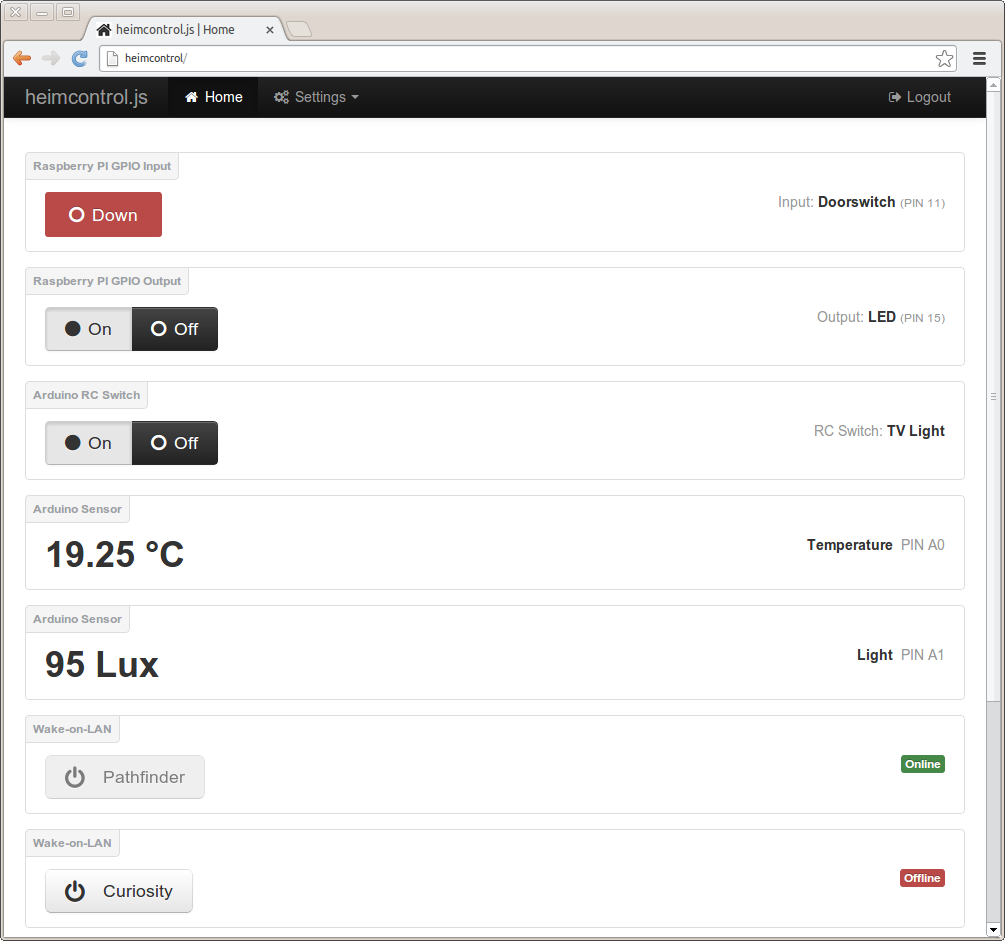
\includegraphics[width=.5\textwidth]{gfx/heimcontrol.png}
			\end{center}

		
		\subsubsection{Quake}
		
			Not really a resource but you can play Quake on a Raspberry Pi.
			Damned cool.
			
		
		\subsubsection{RPi Cam Web Interface}

			This program allows you to stream a live feed from the RPi Camera module( or USB webcam ) to a webpage (hosted by the Pi) at a respectable FPS (around 15) . The feed can be accessed by any web browser. The program also allows high-defintion video recording, motion dectection and image capturing. This program can be used for home surveillance purposes. There is currently a prototype built complete with web controlled servos which allows for tilt and pan movements.

			\end{multicols}
			\begin{figure}[H]
				\centering
				\caption{RPi Camera Web Interface Prototype.}
				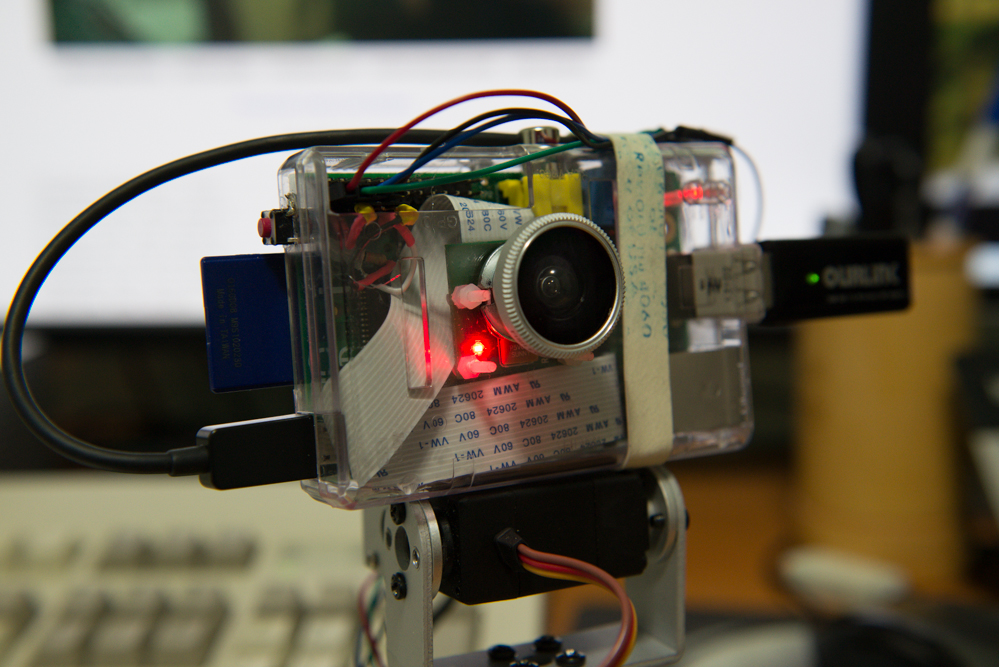
\includegraphics[width=.45\textwidth]{gfx/picam.jpg} 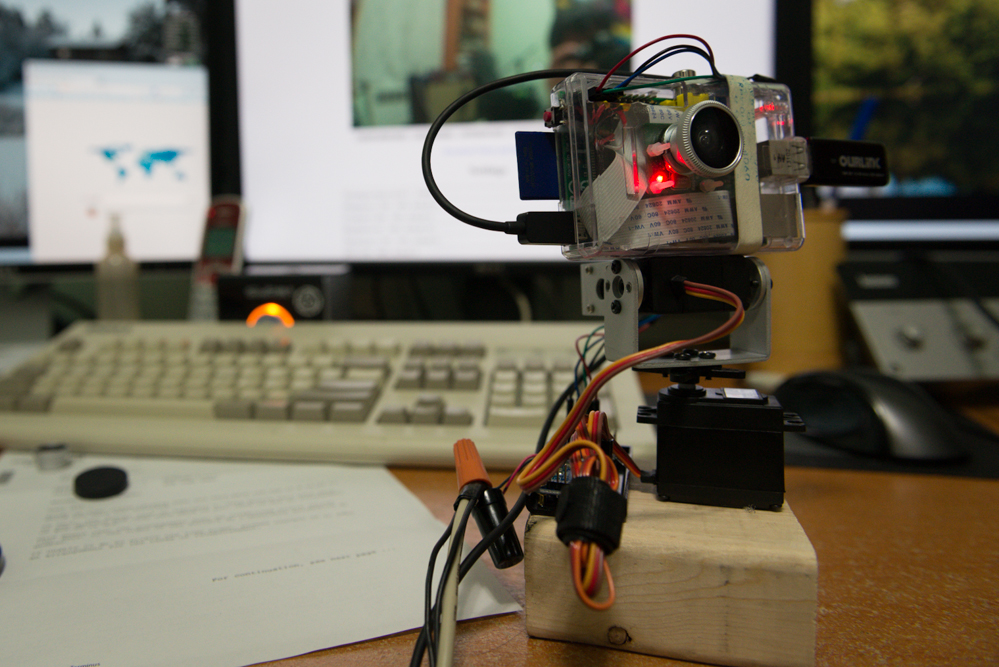
\includegraphics[width=.45\textwidth]{gfx/picam2.jpg}
				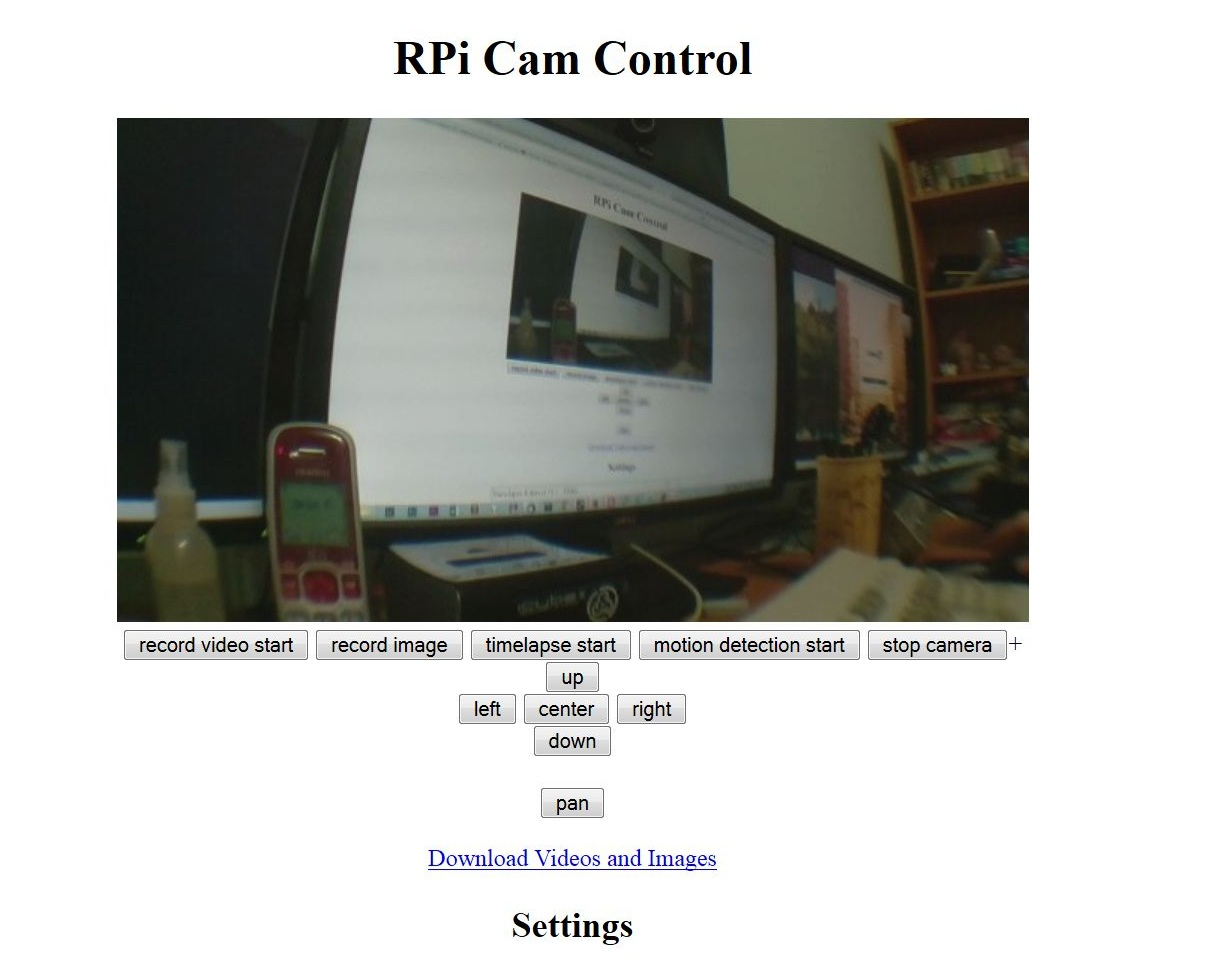
\includegraphics[width=0.6\textwidth]{gfx/picam3.jpg}
				\end{figure}
			\begin{multicols}{2}
		
		
			
\section{Strategy}

	\subsection{Behaviour Modification and Working Toward a Better Society}
			
			
\section{Cost Analysis}

	\subsection{Raspberry Pi Satellites}
	
	\subsection{Server}
	
	\subsection{Arduino Automation}
	
	\subsection{Load Balancing}
	
		The following has been assembled as a bill of materials for load balancing. \\
		\begin{tabular}{r|l}
			39.00 &	1 Spark Core Wireless \href{https://www.spark.io}{transceiver/microprocessor} \\
			29.70 & 3  Spark \href{http://oshpark.com/shared_projects/E1XSjK44}{relay/power monitor shields} \\
			04.00 & jumper wires
		\end{tabular}
		
\section{Conclusion}

	Hyve's primary endeavour is behaviour modification and a bolder marriage of technology and the home.
	It is through true integration of and comfort with technology that communities can become closer together.
	
	Hyve is designed to both protect the individual, his property, his person, and his privacy, and also to help connect him to his neighbours.
	While I expand this paper, this will be further detailed.

\end{multicols}
\end{document}